\documentclass[tikz,border=8pt]{standalone}
\usepackage{amsmath}
\usepackage{amssymb}
\usepackage{tikz}
\usetikzlibrary{arrows.meta,calc,decorations.pathreplacing,patterns,shapes.geometric,positioning,shadings}

\begin{document}
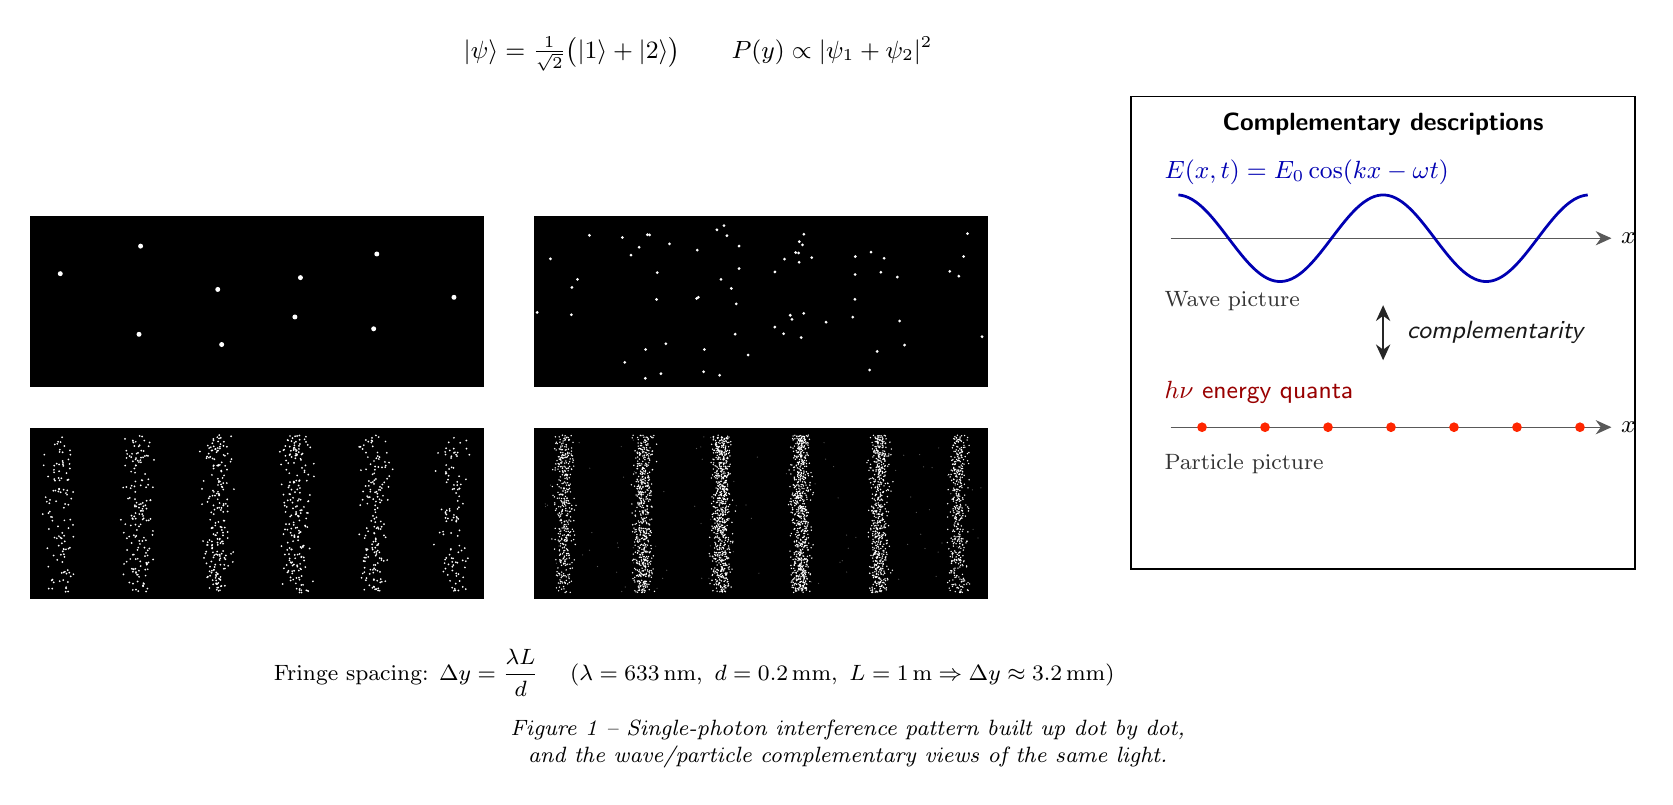
\begin{tikzpicture}[
  >={Stealth[length=2mm,width=1.8mm]},
  font=\sffamily\small,
  screen/.style={draw=white,line width=0.8pt,fill=black},
  framebox/.style={draw=black,line width=0.6pt},
  dotw/.style={circle,fill=white,inner sep=0pt,minimum size=0.6pt},
  photon/.style={circle,fill=red!70!orange,inner sep=0pt,minimum size=3.5pt},
]

%--- Top heading with superposition and probability
\node[anchor=south] at (5.6,6.7) {$|\psi\rangle=\tfrac{1}{\sqrt{2}}\bigl(|1\rangle+|2\rangle\bigr)\qquad P(y)\propto|\psi_{1}+\psi_{2}|^{2}$};

%=====================================================
% LEFT: Four CCD-style sub-panels with shared geometry
%=====================================================
% Shared horizontal fringe positions (in panel local x in cm)
% 6 bright fringes at x = -2.5, -1.5, -0.5, 0.5, 1.5, 2.5 (spacing 1 cm = 3.2 mm)
% Gaussian envelope centered at x=0 with sigma ~ 2.0

% Helper: define bright fringe centers list for foreach
% We'll scatter dots using a cosine^2 * Gaussian acceptance done via several random foreach passes.

% ------- Panel A: N = 10 (very sparse) -------
\begin{scope}[shift={(0,3.9)}]
  \draw[screen] (-2.9,-1.1) rectangle (2.9,1.1);
  % 10 dots: place near fringe centers with small random offsets
  \foreach \cx/\cy in {-2.5/0.35, -1.5/-0.42, -0.5/0.15, -0.45/-0.55, 0.55/0.30, 0.48/-0.20, 1.52/0.60, 1.48/-0.35, 2.5/0.05, -1.48/0.70}
    \fill[white] (\cx,\cy) circle (0.9pt);
  \node[white,anchor=north] at (0,-1.15) {$N=10$};
\end{scope}

% ------- Panel B: N = 100 (scattered, faint clusters) -------
\begin{scope}[shift={(6.4,3.9)}]
  \draw[screen] (-2.9,-1.1) rectangle (2.9,1.1);
  % 100 dots, biased toward fringe centers
  \foreach \i in {1,...,100} {
    \pgfmathsetmacro{\fringe}{int(mod(\i,6))}
    \pgfmathsetmacro{\cx}{-2.5+\fringe*1.0}
    \pgfmathsetmacro{\rx}{rnd*0.7-0.35}
    \pgfmathsetmacro{\ry}{rnd*2.0-1.0}
    \pgfmathsetmacro{\env}{exp(-((\cx+\rx)*(\cx+\rx))/8)}
    \pgfmathsetmacro{\acc}{rnd}
    \ifdim \acc pt<\env pt
      \fill[white] (\cx+\rx,\ry) circle (0.55pt);
    \fi
  }
  \node[white,anchor=north] at (0,-1.15) {$N=10^{2}$};
\end{scope}

% ------- Panel C: N = 10,000 (emerging fringes) -------
\begin{scope}[shift={(0,1.2)}]
  \draw[screen] (-2.9,-1.1) rectangle (2.9,1.1);
  % Use many foreach passes centered at fringe maxima with narrow gaussian scatter
  \foreach \cx in {-2.5,-1.5,-0.5,0.5,1.5,2.5} {
    \pgfmathsetmacro{\env}{exp(-(\cx*\cx)/8)}
    \pgfmathsetmacro{\numdots}{int(180*\env+30)}
    \foreach \i in {1,...,\numdots} {
      \pgfmathsetmacro{\rx}{(rnd+rnd+rnd-1.5)*0.18}
      \pgfmathsetmacro{\ry}{rnd*2.0-1.0}
      \fill[white] (\cx+\rx,\ry) circle (0.35pt);
    }
  }
  \node[white,anchor=north] at (0,-1.15) {$N=10^{4}$};
\end{scope}

% ------- Panel D: N = 1,000,000 (crisp fringes) -------
\begin{scope}[shift={(6.4,1.2)}]
  \draw[screen] (-2.9,-1.1) rectangle (2.9,1.1);
  % Dense vertical stripes with gaussian envelope
  \foreach \cx in {-2.5,-1.5,-0.5,0.5,1.5,2.5} {
    \pgfmathsetmacro{\env}{exp(-(\cx*\cx)/8)}
    \pgfmathsetmacro{\numdots}{int(600*\env+120)}
    \foreach \i in {1,...,\numdots} {
      \pgfmathsetmacro{\rx}{(rnd+rnd+rnd+rnd-2.0)*0.10}
      \pgfmathsetmacro{\ry}{rnd*2.0-1.0}
      \fill[white] (\cx+\rx,\ry) circle (0.28pt);
    }
  }
  % extra fill between fringes (low density)
  \foreach \i in {1,...,120} {
    \pgfmathsetmacro{\rx}{rnd*5.6-2.8}
    \pgfmathsetmacro{\ry}{rnd*2.0-1.0}
    \fill[white,opacity=0.35] (\rx,\ry) circle (0.22pt);
  }
  \node[white,anchor=north] at (0,-1.15) {$N=10^{6}$};
\end{scope}

%--- Geometry callout under left block
\node[anchor=north,align=center,font=\footnotesize] at (5.6,-0.4) {
  Fringe spacing: $\Delta y=\dfrac{\lambda L}{d}$ \quad
  ($\lambda=633\,\mathrm{nm},\ d=0.2\,\mathrm{mm},\ L=1\,\mathrm{m}\Rightarrow \Delta y\approx 3.2\,\mathrm{mm}$)
};

%=====================================================
% RIGHT small figure: wave vs. photons + complementarity
%=====================================================
\begin{scope}[shift={(14.3,3.5)}]
  % outer white panel
  \draw[framebox,fill=white] (-3.2,-3.0) rectangle (3.2,3.0);

  % Title
  \node at (0,2.65) {\textbf{Complementary descriptions}};

  % --- Wave (top) ---
  \begin{scope}[shift={(0,1.2)}]
    \draw[->,gray!70!black] (-2.7,0) -- (2.9,0) node[right,black] {$x$};
    \draw[blue!70!black,line width=1.0pt,domain=-2.6:2.6,samples=120,smooth]
      plot (\x, {0.55*cos(deg(\x*2.4))});
    \node[blue!70!black,anchor=south west] at (-2.9,0.55) {$E(x,t)=E_0\cos(kx-\omega t)$};
    \node[anchor=north west,gray!40!black,font=\footnotesize] at (-2.9,-0.55) {Wave picture};
  \end{scope}

  % --- Double-headed arrow + "complementarity" ---
  \draw[<->,line width=0.9pt,gray!30!black] (0,0.35) -- (0,-0.35);
  \node[anchor=west,gray!20!black] at (0.18,0) {\itshape complementarity};

  % --- Photons (bottom) ---
  \begin{scope}[shift={(0,-1.2)}]
    \draw[->,gray!70!black] (-2.7,0) -- (2.9,0) node[right,black] {$x$};
    \foreach \x in {-2.3,-1.5,-0.7,0.1,0.9,1.7,2.5}
      \node[photon] at (\x,0) {};
    \node[anchor=south west,red!60!black] at (-2.9,0.18) {$h\nu$ energy quanta};
    \node[anchor=north west,gray!40!black,font=\footnotesize] at (-2.9,-0.22) {Particle picture};
  \end{scope}
\end{scope}

%--- Title (rendered as sub-caption at bottom, kept in English for TikZ)
\node[anchor=north,align=center,font=\footnotesize\itshape] at (7.5,-1.3)
  {Figure 1 -- Single-photon interference pattern built up dot by dot,\\
   and the wave/particle complementary views of the same light.};

\end{tikzpicture}
\end{document}
